\chapter{Ensayos de Validaciones} \label{c:ensayo_validacion}
Los ensayos se realizarón con certificados emitidos por la  Secretaría de Extensión de la \gls{fce} de la \gls{unam}, por una cuestión
de conveniencia en el acceso de los documentos digitales de la Universidad, pero los ensayos se podrían realizar sin importancia del área.


El ensayo inicia con la cuenta o dirección del propietario del smart contract, quien  carga los datos base, como el nombre de la Organización, las áreas, los eventos en donde se emitirán los certificados.
Partiendo de un smart contract desplegado como se muestra en otras secciones, el administrador o propietario de la organización es la misma   dirección que se encargó  
de publicar el contrato inteligente, pero el usuario administrador puede cambiar su dirección por otra.
\section{Preparación Inicial}
Los siguientes pasos se realizan con la cuenta del propietario del Smart Contract.
Primero se ingresa el nombre de la organización a “Universidad Nacional de Misiones Facultad de Ciencias Económicas”, esto sirve para identificar el nombre de la organización 
que es dueño del Smart Contract, se 
crean estados nuevos como “en espera”, “on hold” \ref{img:cambio_org}.
Se crean las Áreas de la Organización, es este caso “Secretaría de Extensión”, con el propietario del área con dirección  “0x255A43ac4ed05F41396 07B33523a591ACE5a4031”
y el estado “actived”, conforme a la figura \ref{img:nuva_area}. El propietario del área puede crear las actividades o eventos y realizar la validación de los 
documentos.

\begin{figure}[H]
  \centering
  {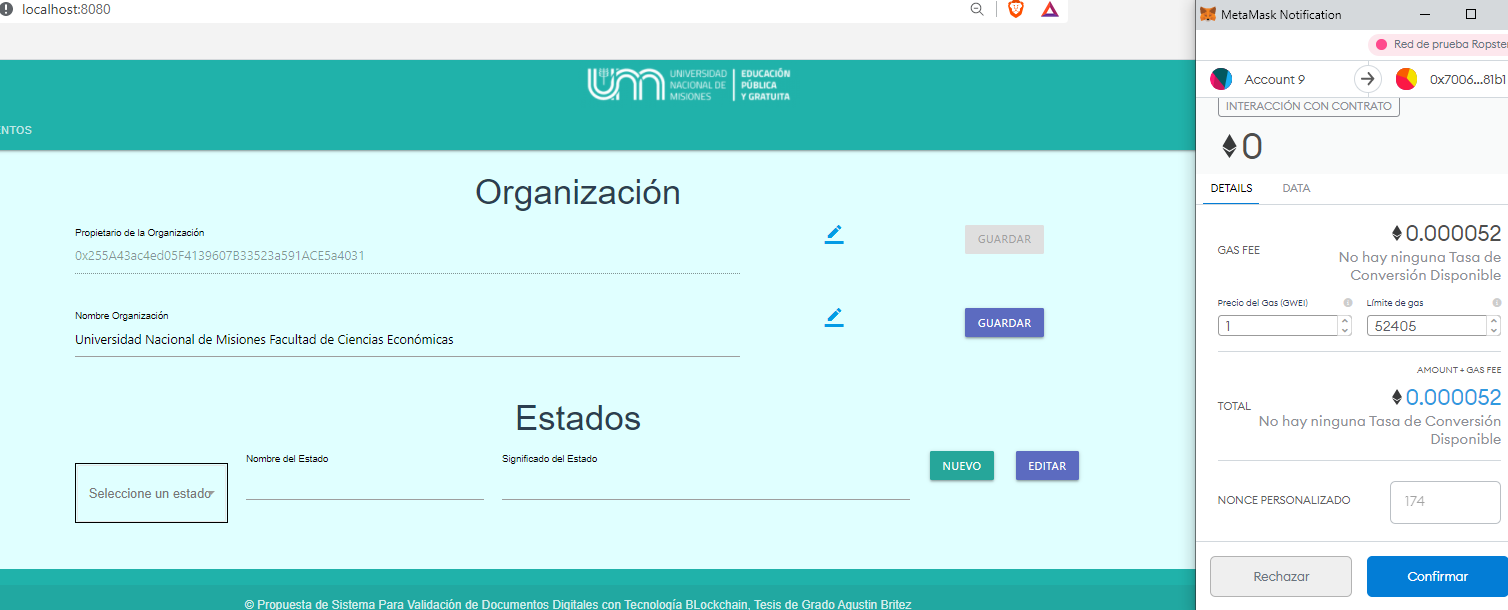
\includegraphics[scale=0.4]{cambio_organizacion.png}}
  \caption{Cambio de nombre de la organización,  Fuente: captura de pantalla. }
  \label{img:cambio_org}
\end{figure}

\begin{figure}[H]
  \centering
  {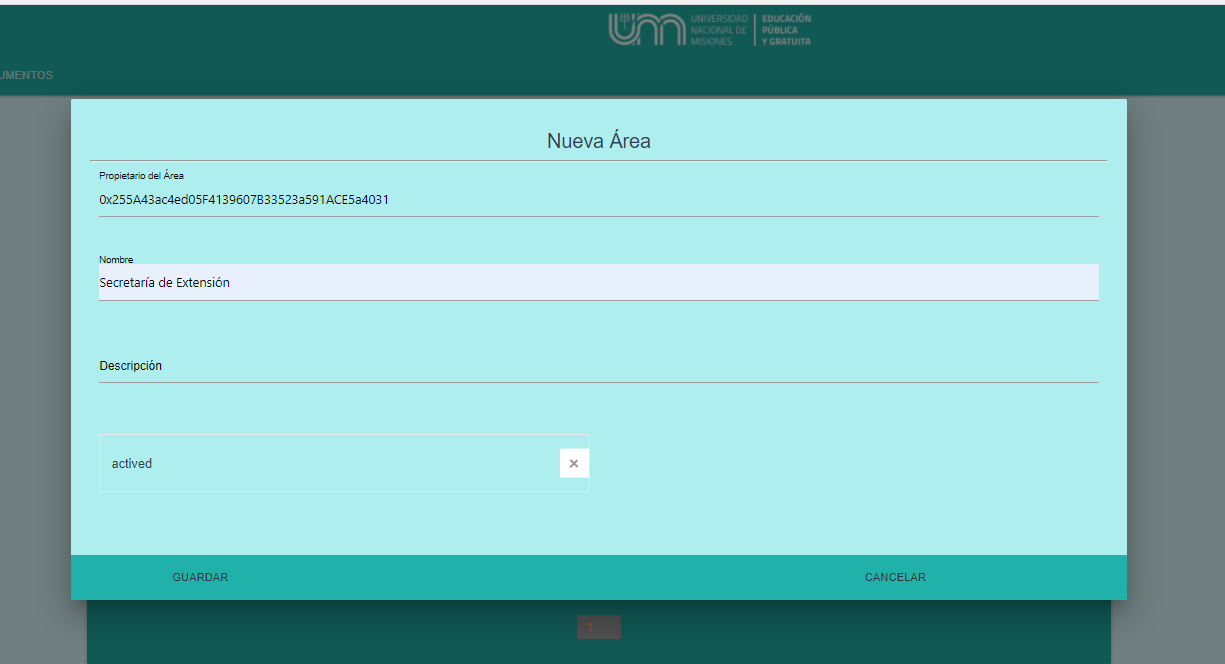
\includegraphics[scale=0.4]{nueva_area.png}}
  \caption{Creación de nueva área en el sistema,  Fuente: captura de pantalla. }
  \label{img:nuva_area}
\end{figure}


Se  crean los  eventos “Fondos Buitres”, “Geogebra” y “Taller  Liquidación”, que se relacionan al área recién mencionada que es 
“Secretaría de Extensión”.
% \begin{figure}[H]
%   \centering
%   {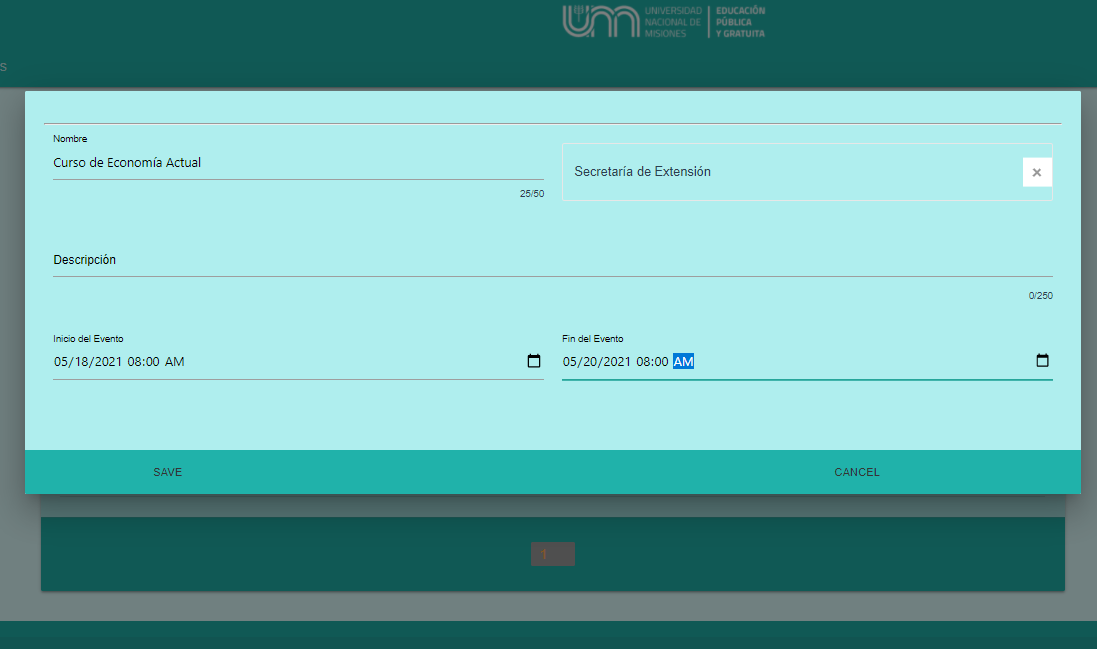
\includegraphics[scale=0.4]{nuevo_evento.png}}
%   \caption{Creación de nueva área en el sistema,  Fuente: captura de pantalla. }
%   \label{img:nuevo_evento}
% \end{figure}


Los ensayos serán realizados con la cuenta del propietario del Smart Contract.

\section{Ensayo A}
Se ensayó en un flujo habitual de la Secretaría de Extensión de la \glsfirst{fce}, 
siguiendo los circuitos normales de una actividad realizada por esta área. En base a la información recaudada en la entrevistas (A.L., comunicación personal, 02/10/2020),
  comenzando el flujo desde el momento que se crea un documento digital para entregar 
al participante de una actividad.

Una vez que el evento haya finalizado y se deben entregar los certificados, estos tiene que ser subidos al sistema de validación de la siguiente manera.
%%aca explicar con el primer certificado como se sube y en que vista o roles estoy
\begin{figure}[H]
  \centering
  {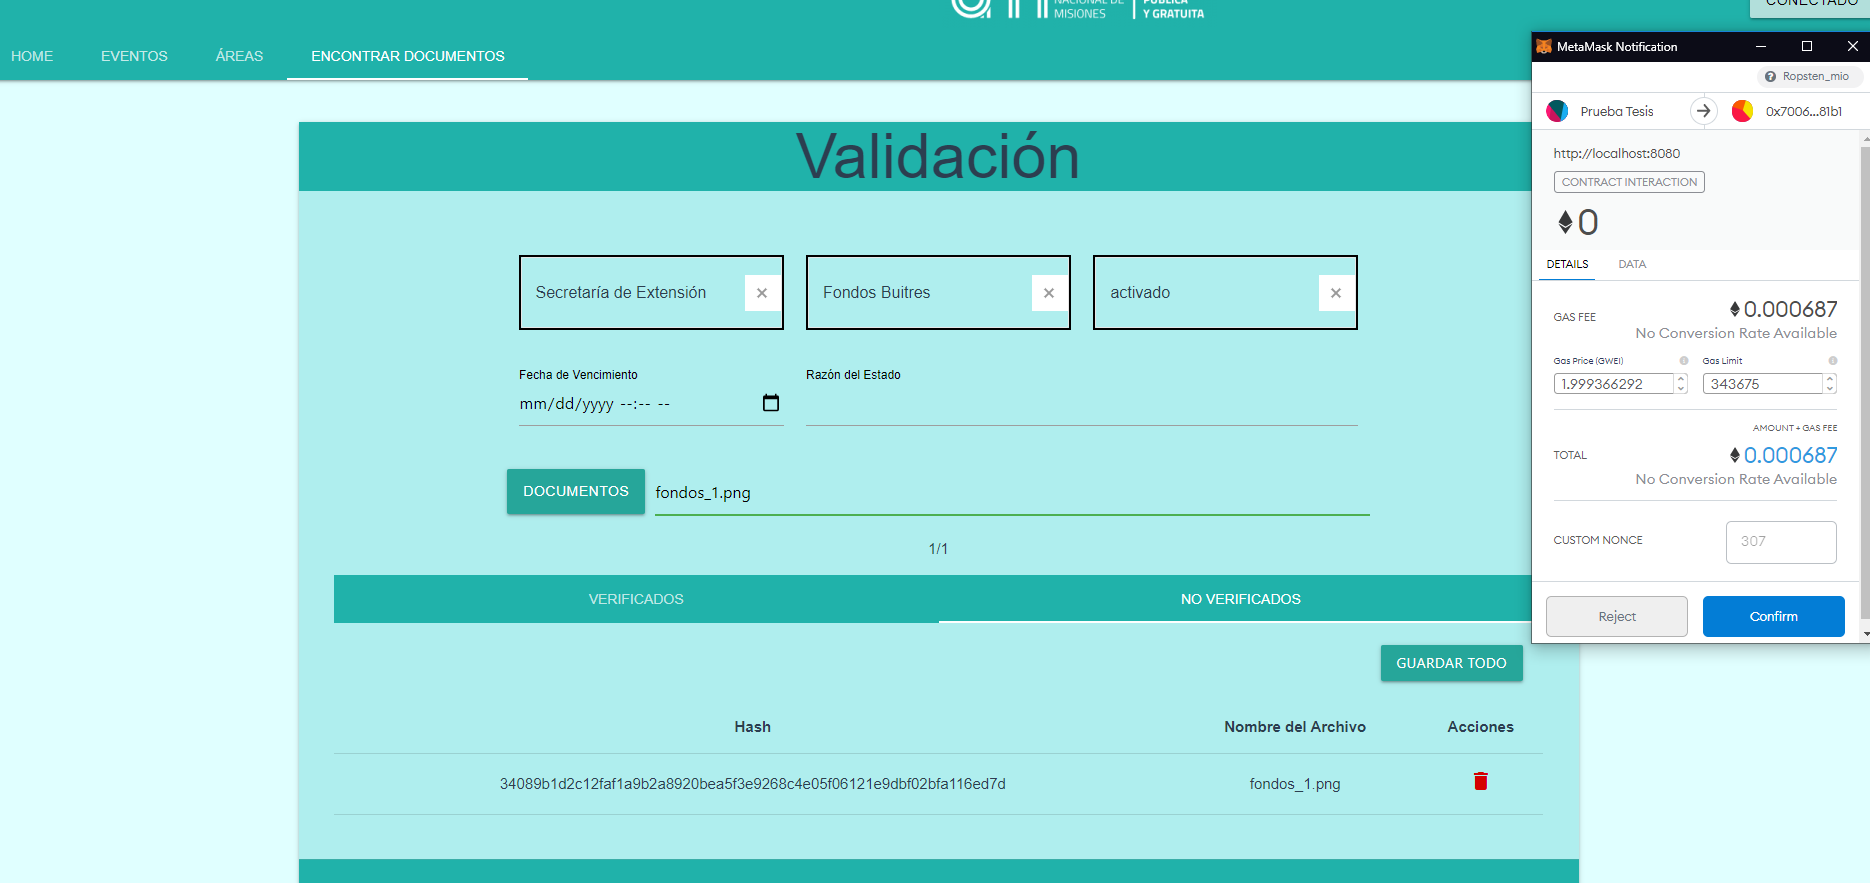
\includegraphics[scale=0.3]{paso_1_subir_documento.png}}
  \caption{Carga de certificado Fondos Buitres,  Fuente: captura de pantalla. }
  \label{img:paso_1}
\end{figure}

\begin{enumerate}
  \item Ingresar al sistema con la cuenta de administrador del área que organiza el evento y dirigirse a la vista “encontrar documento”, en la parte superior del sistema se puede observar en la figura \ref{img:paso_1}.
  \item Seleccionar el área que en este caso es la Secretaría de Extensión.
  \item Seleccionar el evento, en el caso actual es Fondos Buitres y seleccionar el estado que se requiere para los documentos a subir, por ejemplo  el estado “activado”.
  \item Hacer clic en el botón  “documentos” y se busca el certificado a subir en este caso es llamado fondos\_1.png, el certificado se muestra en la figura \ref{img:fondos_1}.
  \item En la figura \ref{img:paso_1} muestra el momento antes de generar el hash y almacenarlo en la Blockchain, cuando el propietario del área presiona el botón “GUARDAR TODO”,el sistema
  genera el hash de  los documentos
  seleccionados que están en la parte de “NO VERIFICADOS” y lo almacena en la Blockchain.
  \item A partir del punto cualquier individuo que consulte la Blockchain podrá verificar que el certificado actual fue emitido por la Secretaría de Extensión de la \gls{fce}. 
\end{enumerate}

\begin{figure}[H]
  \centering
  {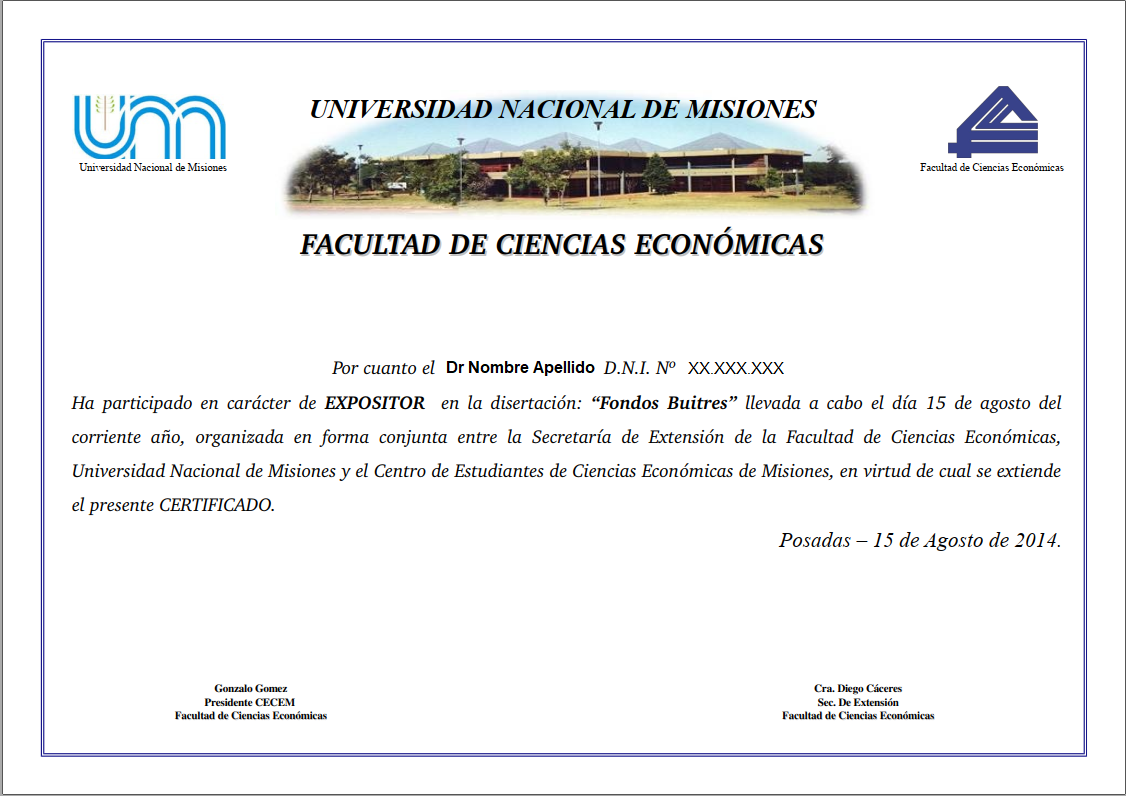
\includegraphics[scale=0.5]{Certificados Originales/fondos_1.png}}
  \caption{Certificado Original de fondos buitres,  Fuente: captura de pantalla. }
  \label{img:fondos_1}
\end{figure}

En el caso que un interesado desea comprobar que el PDF o documento que esta tiene en su poder fue emitido por la Secretaría de Extensión de la \gls{fce} de la \gls{unam}.
Debe ingresar al sistema en el caso de no ser propietario del área o del smart contract la vista aparece como la figura \ref{img:front_document_public},
luego seleccionar el botón “DOCUMENTOS” y subir el certificado que se quiere validar que es fondos\_1.png 

\begin{figure}[H]
  \centering
  {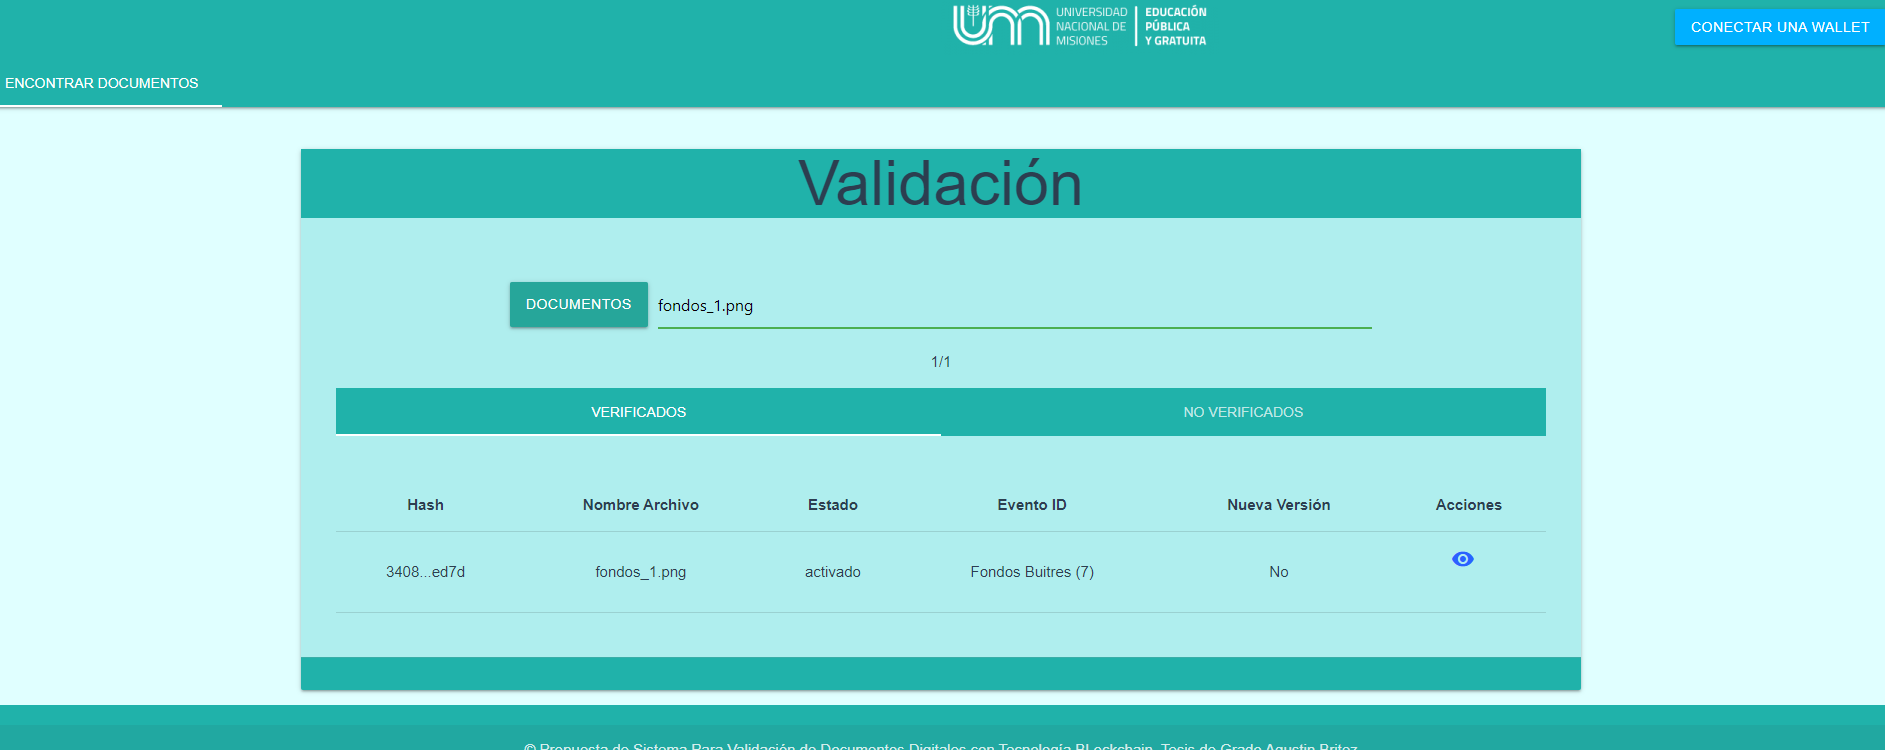
\includegraphics[scale=0.3]{fondos_buitres_captura_verificado.png}}
  \caption{Confirmación que el certificado se encuentra en la blockchain,  Fuente: captura de pantalla. }
  \label{img:fondos_1_verificado}
\end{figure}

Sí una persona intenta modificar el certificado para sus propios beneficios o para 
ocasionar algún tipo de daño de reputación u otro caso, el sistema se encargará de separar los certificados que no fueron emitidos
por una cuenta de propietario de  área de la \gls{fce} o del propietario del smart contract. A continuación el certificado de la figura \ref{img:fondos_1} fue modificado como se muestra en la 
figura \ref{img:fondos_1_alterado} se cambió el nombre del participante del evento a “Dr Ezequiel Britez DNI 00.134.321” (el nombre y el DNI del nuevo participante son
arbitrarios y ficticios). Este es un posible caso el cual una persona necesite un certificado con características esenciales para ella y modifique 
el documento a su voluntad.

\begin{figure}[H]
  \centering
  {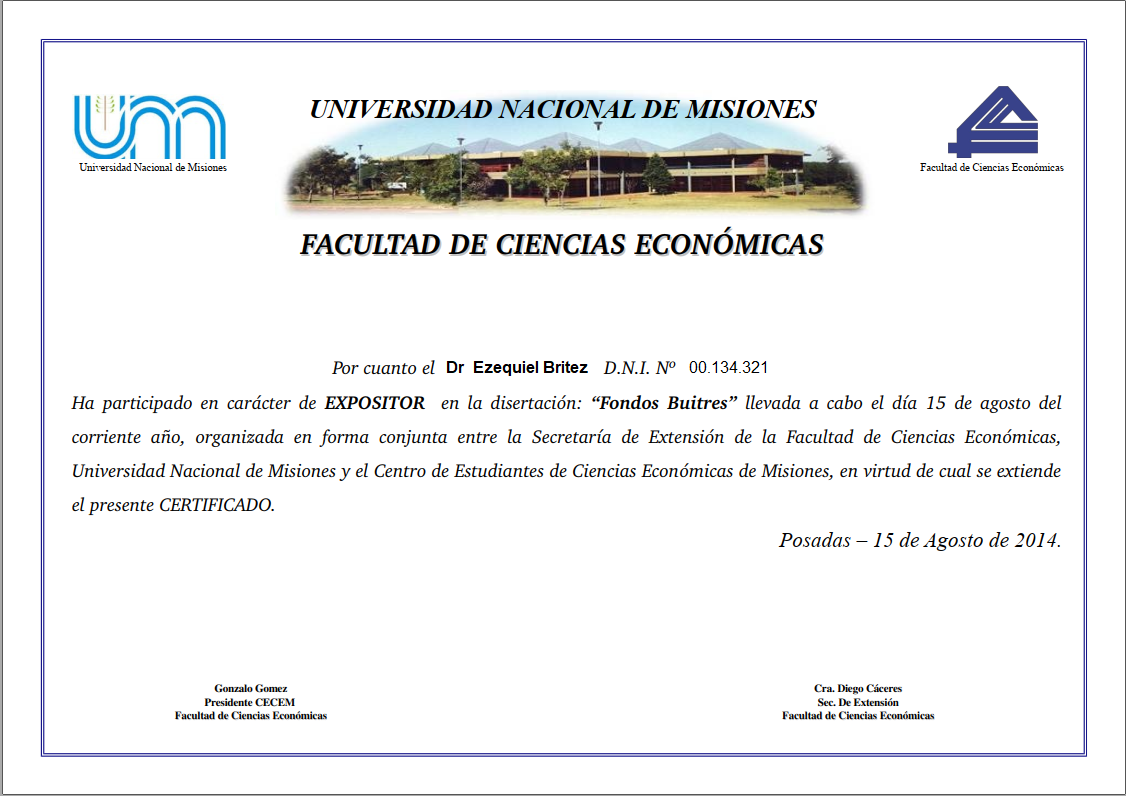
\includegraphics[scale=0.5]{Certificados Originales/fondos_1_alterado.png}}
  \caption{Certificado Fondos Buitres Modificado,  Fuente: captura de pantalla. }
  \label{img:fondos_1_alterado}
\end{figure}

En el caso que el certificado sea presentado, a una entidad podrá verificar  
que los datos
del certificado son correctos. Para ello la entidad debe acceder al sistema y realizar el 
mismo ya explicado, el cual es subir el documento
con el botón “DOCUMENTOS” de la vista. Para saber que el certificado o documento mantiene su información inalterable y que es emitida por la \gls{fce} de la \gls{unam},
el hash del certificado aparece en la sección “VERIFICADOS” como se muestra en la figura \ref{img:fondos_1_modificado_validacion}.

\begin{figure}[H]
  \centering
  {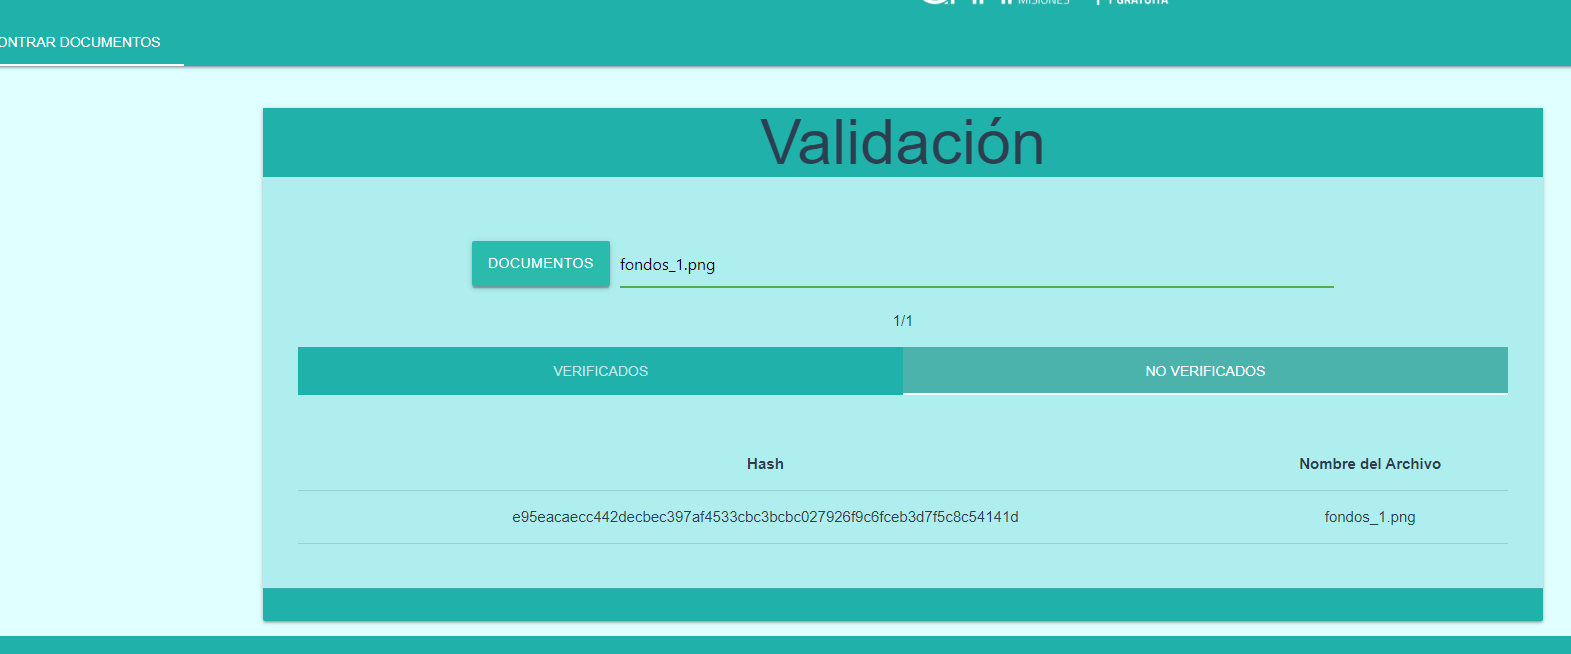
\includegraphics[scale=0.4]{fondos_1_prueba_modificado.png}}
  \caption{Validación de certificado modificado,  Fuente: captura de pantalla. }
  \label{img:fondos_1_modificado_validacion}
\end{figure}

Como se puede observar la tabla  \ref{table:tabla-ensayo-a} el hash del documento modificado es distinto al documento original.

\begin{table}[H]
  \centering
  % l = lefht c=centrado r=right
  \begin{tabular}{ |l|l|l| }
  \hline
  Hash Original & Hash Modificado & Cambia \\
  \hline
  34089b1d2c12faf1a9b2a8920 & e95eacaecc442decbec397af  &    \\
  bea5f3e9268c4e05f06121e9d & 4533cbc3bcbc027926f9c6fc  & SI \\
  bf02bfa116ed7d            & eb3d7f5c8c54141d          &    \\
  \hline
  \end{tabular}
  \caption{Comparación de los hash del certificado original \ref{img:fondos_1} y el modificado \ref{img:fondos_1_alterado}  }
  \label{table:tabla-ensayo-a}
  \end{table}

El resultado son distintos hashes porque los bits de cada documento son distintos \cite[]{back_hashcash_2002,nakamoto_bitcoin_2008,blockcerts_faq_nodate}. 

\section{Ensayo B}
Se sometió a prueba el certificado  (Certificado\_Geogebra.png de la figura \ref{img:certificado_geogebra}),
donde se cargan los datos Área: Secretaría de Extensión, Evento: Geogebra y Estado: Activado.
Y de la misma manera que el Ensayo A se carga el documento y confirma la transacción.

\begin{figure}[H]
  \centering
  {
\includegraphics[scale=0.5]{Certificados Originales/Certificado_Geogebra.png}}
  \caption{Certificado de participación curso Geogebra,  Fuente: captura de pantalla. }
  \label{img:certificado_geogebra}
\end{figure}

Es observable  en la figura \ref{img:geogebra_validado} que el certificado se subió correctamente y el hash se genero.

\begin{figure}[H]
  \centering
  {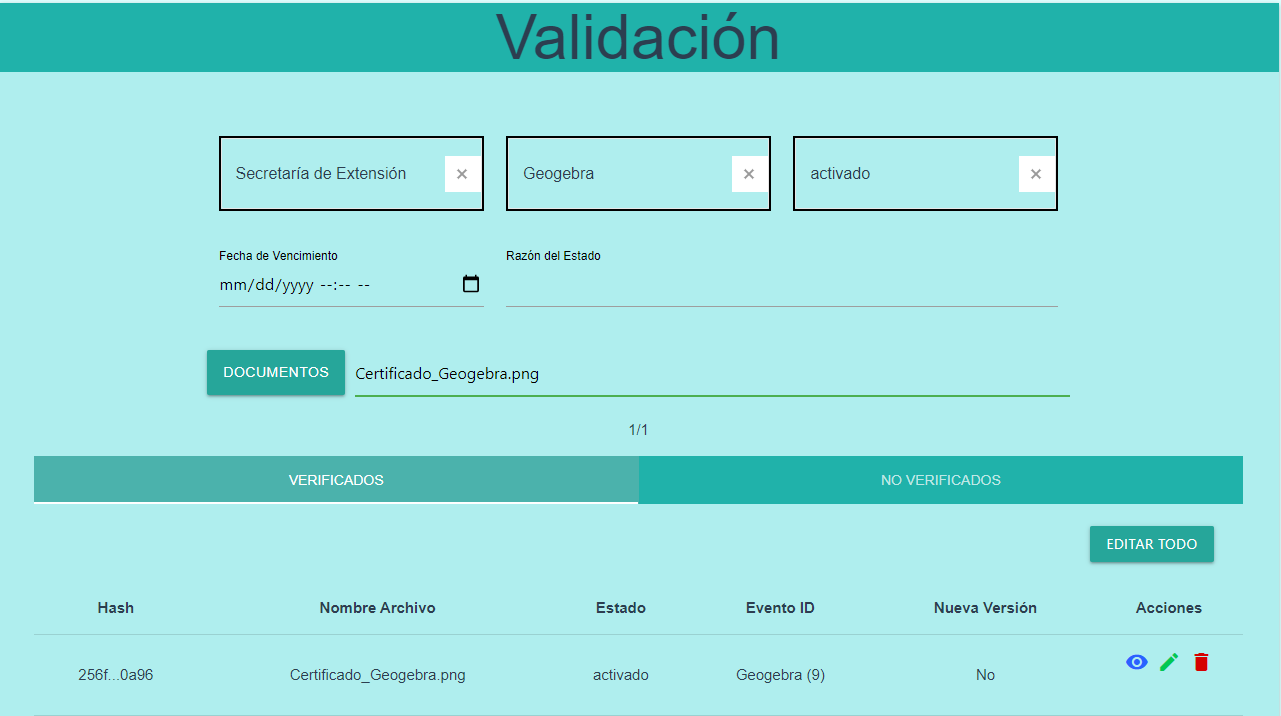
\includegraphics[scale=0.5]{geogebra_validado.png}}
  \caption{Certificado de Geogebra Validado,  Fuente: captura de pantalla. }
  \label{img:geogebra_validado}
\end{figure}

Como prueba se cambió el nombre del archivo de Certificado\_Geogebra.png a Bartolomeo\_Certificado\_Geo.png (ver Figura \ref{img:geogebra_cambio_nombre}) 
y se sometió al sistema 
para conocer si la integridad del certificado cambió. 

El  certificado aparece en la sección “VERIFICADOS” tras cambiar el nombre del archivo y probarlo. El sistema 
verifica que el hash del documento no 
se modificó porque internamente no sufrió cambios, esto permite  realizar modificaciones en el nombre del documento y no alterar a la validación.

\begin{figure}[H]
  \centering
  {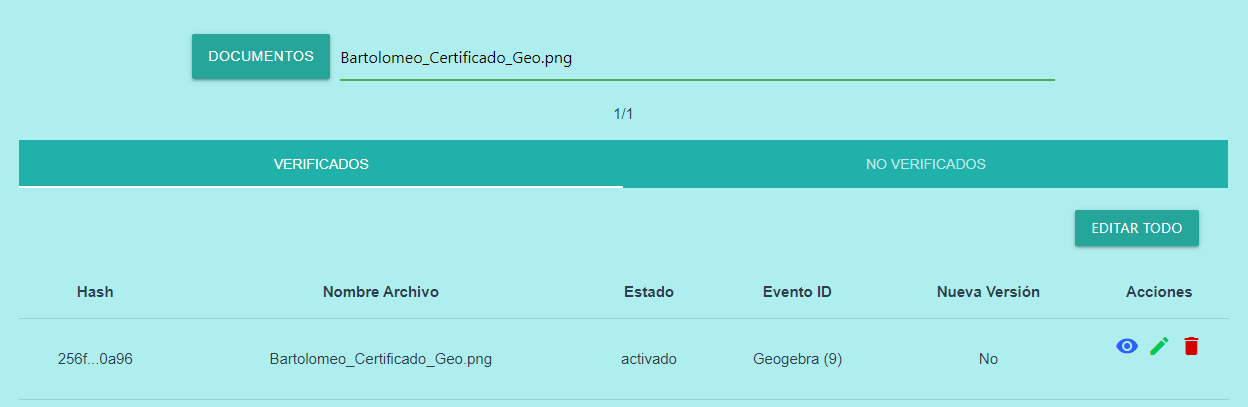
\includegraphics[scale=0.5]{geo_cambio_nombre.png}}
  \caption{Cambio de nombre del Certificado,  Fuente: captura de pantalla. }
  \label{img:geogebra_cambio_nombre}
\end{figure}

A continuación se realiza una modificaciones internas  del Certificado\_Geogebra.png y el resultado se muestra en la figura  \ref{img:geogebra_alterado}

\begin{figure}[H]
  \centering
  {
\includegraphics[scale=0.5]{Certificados Originales/Geogebra_1_alterado.png}}
  \caption{Certificado de Geogebra No Validado,  Fuente: captura de pantalla. }
  \label{img:geogebra_alterado}
\end{figure}

En la figura \ref{img:geogebra_alterado} se modificó el año del evento,  en algunas ocasiones las personas requieren
demostrar que realizó una capacitación o que tienen las habilidades que el certificado
demuestra. O cuando necesitan tener años de experiencias podría ocurrir un cambio de fechas.

Se probó el certificado modificado con el mismo nombre archivo pero este último no afecta al cálculo del hash. La prueba se muestra en
la figura \ref{img:geogebra_alterado_prueba} 

\begin{figure}[H]
  \centering
  {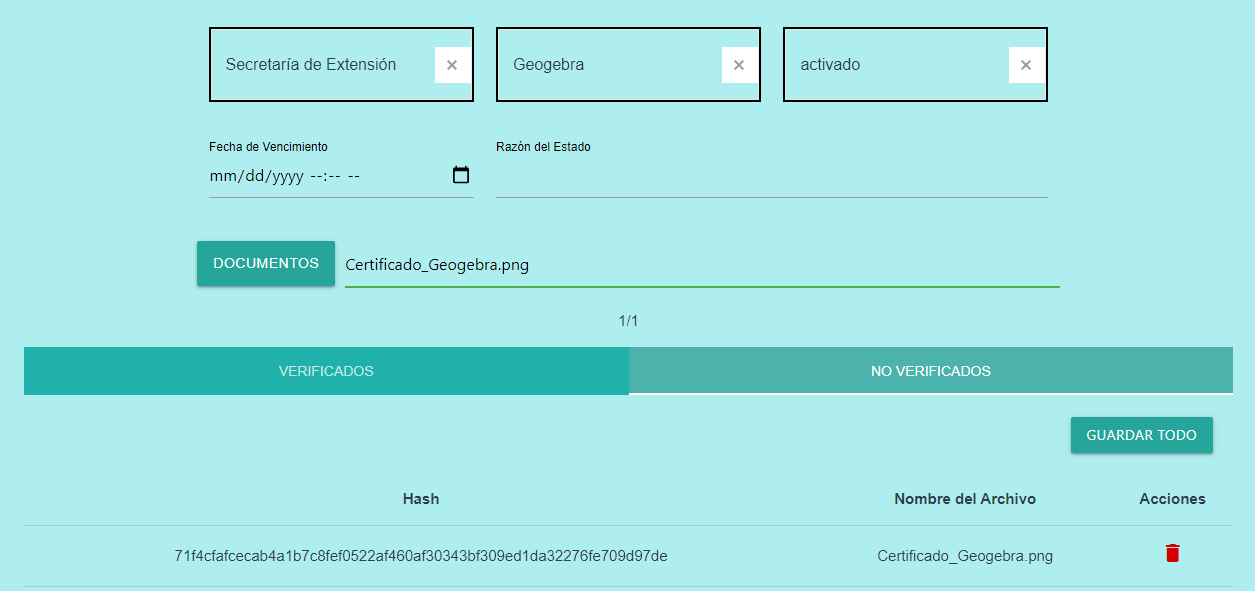
\includegraphics[scale=0.4]{geo_validacion_alterado.png}}
  \caption{Certificado de Geogebra Validado,  Fuente: captura de pantalla. }
  \label{img:geogebra_alterado_prueba}
\end{figure}

Como resultado se detectó que el HASH cambió por ende el certificado aparece en el sector “NO VERIFICADOS”.
Con la tabla \ref{table:tabla-ensayo-b} se puede observar la diferencias entre los hashes.

\begin{table}[H]
  \centering
  % l = lefht c=centrado r=right
  \begin{tabular}{ |l|l|l| }
  \hline
  Hash Original              & Hash Modificado          & Cambia \\
  \hline
  256f5c768d464033868cede3a & 71f4cfafcecab4a1b7c8fef0  &    \\
  e62dffbe3c506ceed9079b951 & 522af460af30343bf309ed1d  & SI \\
  f08b4b3bd00a96            & a32276fe709d97de          &    \\
  \hline
  \end{tabular}
  \caption{Comparación de los hash del certificado original \ref{img:certificado_geogebra} y el modificado \ref{img:geogebra_alterado}  }
  \label{table:tabla-ensayo-b}
  \end{table}

  \section{Ensayo C}
  Se sometió a prueba el certificado  (Certificado\_Liquidación\_ingresos\_brutos.png de la figura \ref{img:certificado_liquidacion}),
donde se cargan los datos Área: Secretaría de Extensión, Evento: Taller Liquidación y Estado: Activado.
De la misma manera que el Ensayo A y B se carga el documento y confirma la transacción.

  \begin{figure}[H]
    \centering
    {\includegraphics[scale=0.5]{Certificados Originales/Certificado_Liquidación_ingresos_brutos.png}}
    \caption{Certificado original del Curso de  Liquidación e Ingresos  Brutos,  Fuente: captura de pantalla. }
    \label{img:certificado_liquidacion}
  \end{figure}

Se realiza el mismo proceso donde se valida el certificado (ver figura \ref{img:liquidacion_validacion}).

\begin{figure}[H]
  \centering
  {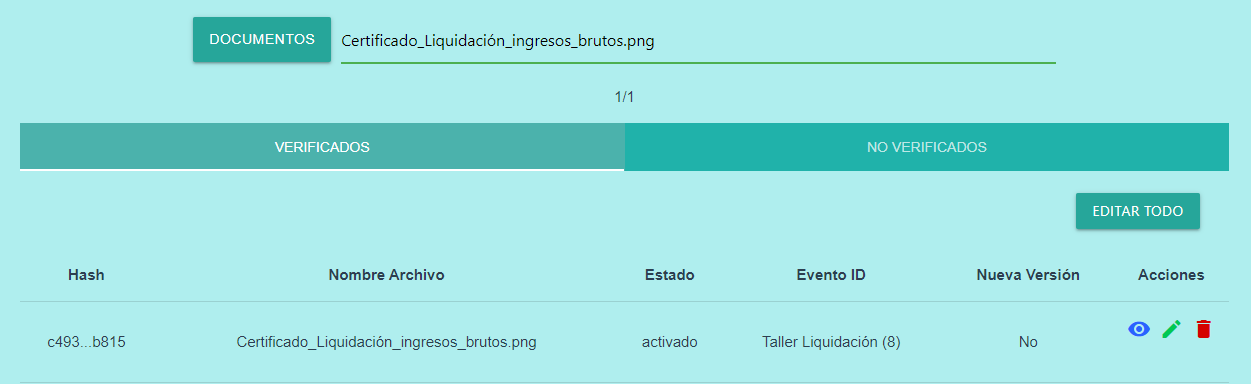
\includegraphics[scale=0.4]{liquidacion_validacion.png}}
  \caption{Prueba de validación del certificado original,  Fuente: captura de pantalla. }
  \label{img:liquidacion_validacion}
\end{figure}

Se realizó un cambio al nombre y DNI en el certificado como resultado se obtuvo el siguiente certificado (ver figura \ref{img:certificado_liquidacion_alterado})  

\begin{figure}[H]
  \centering
  {\includegraphics[scale=0.5]{Certificados Originales/Certificado_Liquidación_ingresos_brutos_alterado.png}}
  \caption{Certificado alterado del curso de Liquidación e Ingresos Brutos,  Fuente: captura de pantalla. }
  \label{img:certificado_liquidacion_alterado}
\end{figure}

Al probar el certificado en la propuesta de sistema de validación, se obtiene que fue modificado porque el hash cambió,  
observar la tabla \ref{table:tabla-ensayo-c} de los hashes las diferencias.

\begin{table}[H]
  \centering
  % l = lefht c=centrado r=right
  \begin{tabular}{ |l|l|l| }
  \hline
  Hash Original              & Hash Modificado          & Cambia \\
  \hline
  c493819261bd3dc6e88b99637 & 6719b1115644f98048db810f  &    \\
  cdf843f84c1dc7080854b83ec & 0228d4eb19f71f10ecc60b85  & SI \\
  bfc5637153b815            & ecab13992c26be94          &    \\
  \hline
  \end{tabular}
  \caption{Comparación de los hash del certificado original \ref{img:certificado_liquidacion} y el modificado \ref{img:certificado_liquidacion_alterado}  }
  \label{table:tabla-ensayo-c}
  \end{table}

En los tres ensayos se obtuvieron los mismos resultados al modificar internamente los certificados, esto se debe al modificar 1 píxel los bits del 
documento digital cambia por ende la el hash generado es otro, cuando se sube un documento al sistema este genera el hash y los busca en 
el smart contract, si se encuentra almacenado significa que una cuenta de la \gls{fce} de la \gls{unam} se encargó de subirla en algún momento,
en caso contrario no se encontrará el hash por ende el certificado no es válido ya que pudo ser emitido por un ente diferente o persona no autorizada.

\section{Consideraciones Detectadas}
El desarrollo del sistema no confirma que a través de la generación de los hashes  un documento digital sea la única manera de validarlos. 
Los estándares investigados y otros sistemas aplicaban este método.
También hay que considerar que la prueba del sistema se realizó en una  Blockchain de prueba, por ende no se puede confirmar que el sistema funciona en todas las Blockchain. 
Si se requiere su uso es necesario probar que la  Blockchain soporte el lenguaje de programación Solidity.

Se tomaron en cuenta los sistemas ya existentes con los estándares investigados y se optó por utilizar funcionamientos similares en los sistemas y que 
toda la información esté almacenada en la  Blockchain y no solo en el documento.
Los ensayos realizados demuestran que cambiando el nombre del archivo no altera el hash, por ende tolera la modificaciones que no intervienen con 
la integridad del documento.

Por otro lado, la implementación del sistema se puede anexar con un sistema externo que gestione los documentos y los suba de manera automática en la  Blockchain, permitiendo
automatizar todo el proceso.